\hypertarget{gtkcolumnview}{%
\section{GtkColumnView}\label{gtkcolumnview}}

\hypertarget{gtkcolumnview-1}{%
\subsection{GtkColumnView}\label{gtkcolumnview-1}}

GtkColumnView is like GtkListView, but it has multiple columns. Each
column is GtkColumnViewColumn.

\begin{figure}
\centering
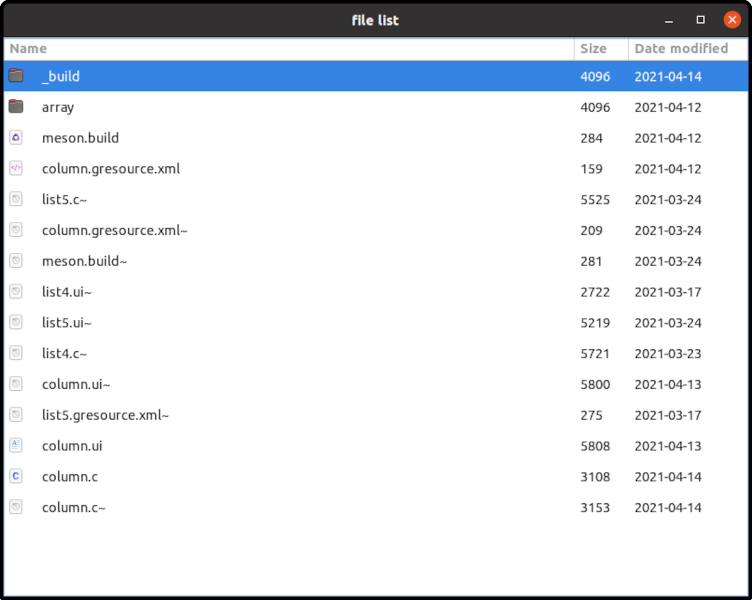
\includegraphics[width=11.3cm,height=9cm]{../image/column_view.png}
\caption{Column View}
\end{figure}

\begin{itemize}
\tightlist
\item
  GtkColumnView has ``model'' property. The property points a
  GtkSelectionModel object.
\item
  Each GtkColumnViewColumn has ``factory'' property. The property points
  a GtkListItemFactory (GtkSignalListItemFactory or
  GtkBuilderListItemFactory).
\item
  The factory connects GtkListItem, which belongs to
  GtkColumnViewColumn, and items of GtkSelectionModel. And the factory
  builds the descendants widgets of GtkColumnView to display the item on
  the display. This process is the same as the one in GtkListView.
\end{itemize}

The following diagram shows the image how it works.

\begin{figure}
\centering
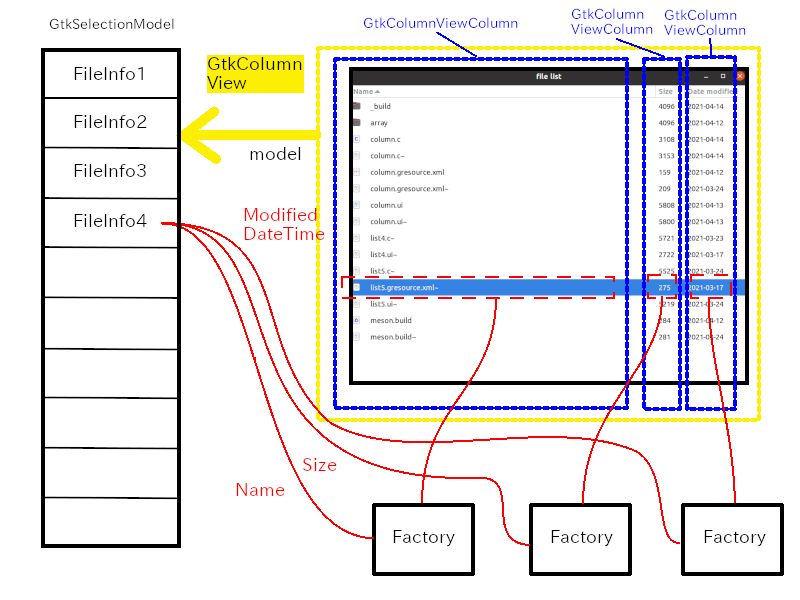
\includegraphics[width=12cm,height=9cm]{../image/column.png}
\caption{ColumnView}
\end{figure}

The example in this section is a window that displays information of
files in a current directory. The information is the name, size and last
modified datetime of files. So, there are three columns.

In addition, the example uses GtkSortListModel and GtkSorter to sort the
information.

\hypertarget{column.ui}{%
\subsection{column.ui}\label{column.ui}}

Ui file specifies whole widgets and their structure.

\begin{lstlisting}[language=XML, numbers=left]
<?xml version="1.0" encoding="UTF-8"?>
<interface>
  <object class="GtkApplicationWindow" id="win">
    <property name="title">file list</property>
    <property name="default-width">800</property>
    <property name="default-height">600</property>
    <child>
      <object class="GtkScrolledWindow" id="scr">
        <property name="hexpand">TRUE</property>
        <property name="vexpand">TRUE</property>
        <child>
          <object class="GtkColumnView" id="columnview">
            <property name="model">
              <object class="GtkSingleSelection" id="singleselection">
                <property name="model">
                  <object class="GtkSortListModel" id="sortlist">
                    <property name="model">
                      <object class="GtkDirectoryList" id="directorylist">
                        <property name="attributes">standard::name,standard::icon,standard::size,time::modified</property>
                      </object>
                    </property>
                    <binding name="sorter">
                      <lookup name="sorter">columnview</lookup>
                    </binding>
                  </object>
                </property>
              </object>
            </property>
            <child>
              <object class="GtkColumnViewColumn" id="column1">
                <property name="title">Name</property>
                <property name="expand">TRUE</property>
                <property name="factory">
                  <object class="GtkBuilderListItemFactory">
                    <property name="bytes"><![CDATA[
<?xml version="1.0" encoding="UTF-8"?>
<interface>
  <template class="GtkListItem">
    <property name="child">
      <object class="GtkBox">
        <property name="orientation">GTK_ORIENTATION_HORIZONTAL</property>
        <property name="spacing">20</property>
        <child>
          <object class="GtkImage">
            <binding name="gicon">
              <closure type="GIcon" function="get_icon_factory">
                <lookup name="item">GtkListItem</lookup>
              </closure>
            </binding>
          </object>
        </child>
        <child>
          <object class="GtkLabel">
            <property name="hexpand">TRUE</property>
            <property name="xalign">0</property>
            <binding name="label">
              <closure type="gchararray" function="get_file_name_factory">
                <lookup name="item">GtkListItem</lookup>
              </closure>
            </binding>
          </object>
        </child>
      </object>
    </property>
  </template>
</interface>
                    ]]></property>
                  </object>
                </property>
                <property name="sorter">
                  <object class="GtkStringSorter" id="sorter_name">
                    <property name="expression">
                      <closure type="gchararray" function="get_file_name">
                      </closure>
                    </property>
                  </object>
                </property>
              </object>
            </child>
            <child>
              <object class="GtkColumnViewColumn" id="column2">
                <property name="title">Size</property>
                <property name="factory">
                  <object class="GtkBuilderListItemFactory">
                    <property name="bytes"><![CDATA[
<?xml version="1.0" encoding="UTF-8"?>
<interface>
  <template class="GtkListItem">
    <property name="child">
      <object class="GtkLabel">
        <property name="hexpand">TRUE</property>
        <property name="xalign">0</property>
        <binding name="label">
          <closure type="gchararray" function="get_file_size_factory">
            <lookup name="item">GtkListItem</lookup>
          </closure>
        </binding>
      </object>
    </property>
  </template>
</interface>
                    ]]></property>
                  </object>
                </property>
                <property name="sorter">
                  <object class="GtkNumericSorter" id="sorter_size">
                    <property name="expression">
                      <closure type="gint64" function="get_file_size">
                      </closure>
                    </property>
                    <property name="sort-order">GTK_SORT_ASCENDING</property>
                  </object>
                </property>
              </object>
            </child>
            <child>
              <object class="GtkColumnViewColumn" id="column3">
                <property name="title">Date modified</property>
                <property name="factory">
                  <object class="GtkBuilderListItemFactory">
                    <property name="bytes"><![CDATA[
<?xml version="1.0" encoding="UTF-8"?>
<interface>
  <template class="GtkListItem">
    <property name="child">
      <object class="GtkLabel">
        <property name="hexpand">TRUE</property>
        <property name="xalign">0</property>
        <binding name="label">
          <closure type="gchararray" function="get_file_time_modified_factory">
            <lookup name="item">GtkListItem</lookup>
          </closure>
        </binding>
      </object>
    </property>
  </template>
</interface>
                    ]]></property>
                  </object>
                </property>
                <property name="sorter">
                  <object class="GtkNumericSorter" id="sorter_datetime_modified">
                    <property name="expression">
                      <closure type="gint64" function="get_file_unixtime_modified">
                      </closure>
                    </property>
                    <property name="sort-order">GTK_SORT_ASCENDING</property>
                  </object>
                </property>
              </object>
            </child>
          </object>
        </child>
      </object>
    </child>
  </object>
</interface>
\end{lstlisting}

\begin{itemize}
\tightlist
\item
  3-12: Widget parent-child relationship is GtkApplicationWindow
  =\textgreater{} GtkScrolledWindow =\textgreater{} GtkColumnView.
\item
  12-18: GtkColumnView has ``model'' property. It points
  GtkSelectionModel interface. In this ui file, GtkSingleSelection is
  used as GtkSelectionModel. GtkSingleSelection is an object that
  implements GtkSelectionModel. And again, it has ``model'' property. It
  points GtkSortListModel. This list model supports sorting the list. It
  will be explained in the later subsection. And it also has ``model''
  property. It points GtkDirectoryList. Therefore, the chain is:
  GtkColumnView =\textgreater{} GtkSingleSelection =\textgreater{}
  GtkSortListModel =\textgreater{} GtkDirectoryList.
\item
  18-20: GtkDirectoryList. It is a list of GFileInfo, which holds
  information of files under a directory. It has ``attributes''
  property. It specifies what attributes is kept in each GFileInfo.

  \begin{itemize}
  \tightlist
  \item
    ``standard::name'' is a name of the file.
  \item
    ``standard::icon'' is a GIcon object of the file
  \item
    ``standard::size'' is the file size.
  \item
    ``time::modified'' is the date and time the file was last modified.
  \end{itemize}
\item
  29-79: The first GtkColumnViewColumn object. There are four
  properties, ``title'', ``expand'', factory" and ``sorter''.
\item
  31: Sets the ``title'' property with ``Name''. This is the title on
  the header of the column.
\item
  32: Sets the ``expand'' property to TRUE to allow the column to expand
  as much as possible. (See the image above).
\item
  33- 69: Sets the ``factory'' property with GtkBuilderListItemFactory.
  The factory has ``bytes'' property which holds a ui string to define a
  template to build GtkListItem composite widget. The CDATA section
  (line 36-66) is the ui string to put into the ``bytes'' property. The
  contents are the same as the ui file
  \passthrough{\lstinline!factory\_list.ui!} in the section 27.
\item
  70-77: Sets the ``sorter'' property with GtkStringSorter object. This
  object provides a sorter that compares strings. It has ``expression''
  property which is set with GtkExpression. A closure tag with a string
  type function \passthrough{\lstinline!get\_file\_name!} is used here.
  The function will be explained later.
\item
  80-115: The second GtkColumnViewColumn object. Its ``title'',
  ``factory'' and ``sorter'' properties are set. GtkNumericSorter is
  used.
\item
  116-151: The third GtkColumnViewColumn object. Its ``title'',
  ``factory'' and ``sorter'' properties are set. GtkNumericSorter is
  used.
\end{itemize}

\hypertarget{gtksortlistmodel-and-gtksorter}{%
\subsection{GtkSortListModel and
GtkSorter}\label{gtksortlistmodel-and-gtksorter}}

GtkSortListModel is a list model that sorts its elements according to a
GtkSorter. It has ``sorter'' property that is set with GtkSorter. The
property is bound to ``sorter'' property of GtkColumnView in line 22 to
24.

\begin{lstlisting}[language=XML]
<object class="GtkSortListModel" id="sortlist">
... ... ...
  <binding name="sorter">
    <lookup name="sorter">columnview</lookup>
  </binding>
\end{lstlisting}

Therefore, \passthrough{\lstinline!columnview!} determines the way how
to sort the list model. The ``sorter'' property of GtkColumnView is
read-only property and it is a special sorter. It reflects the user's
sorting choice. If a user clicks the header of a column, then the sorter
(``sorter'' property) of the column is referenced by ``sorter'' property
of the GtkColumnView. If the user clicks the header of another column,
then the ``sorter'' property of the GtkColumnView refers to the newly
clicked column's ``sorter'' property.

The binding above makes a indirect connection between the ``sorter''
property of GtkSortListModel and the ``sorter'' property of each column.

GtkSorter has several child objects.

\begin{itemize}
\tightlist
\item
  GtkStringSorter compares strings.
\item
  GtkNumericSorter compares numbers.
\item
  GtkCustomSorter uses a callback to compare.
\item
  GtkMultiSorter combines multiple sorters.
\end{itemize}

The example uses GtkStringSorter and GtkNumericSorter.

GtkStringSorter uses GtkExpression to get the strings from the objects.
The GtkExpression is stored in the ``expression'' property of
GtkStringSorter. For example, in the ui file above, the GtkExpression is
in the line 71 to 76.

\begin{lstlisting}[language=XML]
<object class="GtkStringSorter" id="sorter_name">
  <property name="expression">
    <closure type="gchararray" function="get_file_name">
    </closure>
  </property>
</object>
\end{lstlisting}

The GtkExpression calls \passthrough{\lstinline!get\_file\_name!}
function when it is evaluated.

\begin{lstlisting}[language=C, numbers=left]
char *
get_file_name (GFileInfo *info) {
  g_return_val_if_fail (G_IS_FILE_INFO (info), NULL);

  return g_strdup(g_file_info_get_name (info));
}
\end{lstlisting}

The function is given the item (GFileInfo) of the GtkSortListModel as an
argument (\passthrough{\lstinline!this!} object). The function retrieves
a filename from \passthrough{\lstinline!info!}. The string is owned by
\passthrough{\lstinline!info!} so it is necessary to duplicate it. And
it returns the copied string. The string will be owned by the
expression.

GtkNumericSorter compares numbers. It is used in the line 106 to 112 and
line 142 to 148. The lines from 106 to 112 is:

\begin{lstlisting}[language=XML]
<object class="GtkNumericSorter" id="sorter_size">
  <property name="expression">
    <closure type="gint64" function="get_file_size">
    </closure>
  </property>
  <property name="sort-order">GTK_SORT_ASCENDING</property>
</object>
\end{lstlisting}

The closure tag specifies a callback function
\passthrough{\lstinline!get\_file\_size!}.

\begin{lstlisting}[language=C, numbers=left]
goffset
get_file_size (GFileInfo *info) {
  g_return_val_if_fail (G_IS_FILE_INFO (info), -1);

  return g_file_info_get_size (info);
}
\end{lstlisting}

It just returns the size of \passthrough{\lstinline!info!}. The type of
the size is \passthrough{\lstinline!goffset!}. The type
\passthrough{\lstinline!goffset!} is the same as
\passthrough{\lstinline!gint64!}.

The lines from 142 to 148 is:

\begin{lstlisting}[language=XML]
<object class="GtkNumericSorter" id="sorter_datetime_modified">
  <property name="expression">
    <closure type="gint64" function="get_file_unixtime_modified">
    </closure>
  </property>
  <property name="sort-order">GTK_SORT_ASCENDING</property>
</object>
\end{lstlisting}

The closure tag specifies a callback function
\passthrough{\lstinline!get\_file\_unixtime\_modified!}.

\begin{lstlisting}[language=C, numbers=left]
gint64
get_file_unixtime_modified (GFileInfo *info) {
  g_return_val_if_fail (G_IS_FILE_INFO (info), -1);

  GDateTime *dt;

  dt = g_file_info_get_modification_date_time (info);
  return g_date_time_to_unix (dt);
}
\end{lstlisting}

It gets the modification date and time (GDateTime type) of
\passthrough{\lstinline!info!}. Then it gets a unix time from
\passthrough{\lstinline!dt!}. Unix time, sometimes called unix epoch, is
the number of seconds that have elapsed since 00:00:00 UTC on 1 January
1970. It returns the unix time (gint64 type).

\hypertarget{column.c}{%
\subsection{column.c}\label{column.c}}

\passthrough{\lstinline!column.c!} is as follows.

\begin{lstlisting}[language=C, numbers=left]
#include <gtk/gtk.h>

/* functions (closures) for GtkBuilderListItemFactory */
GIcon *
get_icon_factory (GtkListItem *item, GFileInfo *info) {
  GIcon *icon;
  if (! G_IS_FILE_INFO (info))
    return NULL;
  else {
    icon = g_file_info_get_icon (info);
    g_object_ref (icon);
    return icon;
  }
}

char *
get_file_name_factory (GtkListItem *item, GFileInfo *info) {
  if (! G_IS_FILE_INFO (info))
    return NULL;
  else
    return g_strdup (g_file_info_get_name (info));
}

char *
get_file_size_factory (GtkListItem *item, GFileInfo *info) {
  /* goffset is gint64 */
  goffset size;

  if (! G_IS_FILE_INFO (info))
    return NULL;
  else {
    size = g_file_info_get_size (info);
    return g_strdup_printf ("%ld", (long int) size);
  }
}

char *
get_file_time_modified_factory (GtkListItem *item, GFileInfo *info) {
  GDateTime *dt;

  if (! G_IS_FILE_INFO (info))
    return NULL;
  else {
    dt = g_file_info_get_modification_date_time (info);
    return g_date_time_format (dt, "%F");
  }
}

/* Functions (closures) for GtkSorter */
char *
get_file_name (GFileInfo *info) {
  g_return_val_if_fail (G_IS_FILE_INFO (info), NULL);

  return g_strdup(g_file_info_get_name (info));
}

goffset
get_file_size (GFileInfo *info) {
  g_return_val_if_fail (G_IS_FILE_INFO (info), -1);

  return g_file_info_get_size (info);
}

gint64
get_file_unixtime_modified (GFileInfo *info) {
  g_return_val_if_fail (G_IS_FILE_INFO (info), -1);

  GDateTime *dt;

  dt = g_file_info_get_modification_date_time (info);
  return g_date_time_to_unix (dt);
}

/* ----- activate, open, startup handlers ----- */
static void
app_activate (GApplication *application) {
  GtkApplication *app = GTK_APPLICATION (application);
  GFile *file;

  GtkBuilder *build = gtk_builder_new_from_resource ("/com/github/ToshioCP/column/column.ui");
  GtkWidget *win = GTK_WIDGET (gtk_builder_get_object (build, "win"));
  GtkDirectoryList *directorylist = GTK_DIRECTORY_LIST (gtk_builder_get_object (build, "directorylist"));
  g_object_unref (build);

  gtk_window_set_application (GTK_WINDOW (win), app);

  file = g_file_new_for_path (".");
  gtk_directory_list_set_file (directorylist, file);
  g_object_unref (file);

  gtk_widget_show (win);
}

static void
app_startup (GApplication *application) {
}

#define APPLICATION_ID "com.github.ToshioCP.columnview"

int
main (int argc, char **argv) {
  GtkApplication *app;
  int stat;

  app = gtk_application_new (APPLICATION_ID, G_APPLICATION_FLAGS_NONE);

  g_signal_connect (app, "startup", G_CALLBACK (app_startup), NULL);
  g_signal_connect (app, "activate", G_CALLBACK (app_activate), NULL);
/*  g_signal_connect (app, "open", G_CALLBACK (app_open), NULL);*/

  stat =g_application_run (G_APPLICATION (app), argc, argv);
  g_object_unref (app);
  return stat;
}
\end{lstlisting}

\begin{itemize}
\tightlist
\item
  4-47: Functions for the closure tag in the ``bytes'' property of
  GtkBuilderListItemFactory. These are almost same as the functions in
  section 26 and 26.
\item
  50-72: Functions for the closure in the expression property of
  GtkStringSorter or GtkNumericSorter.
\item
  75-92: \passthrough{\lstinline!app\_activate!} is an ``activate''
  handler of GApplication.
\item
  80-83: Builds objects with ui resource and gets
  \passthrough{\lstinline!win!} and
  \passthrough{\lstinline!directorylist!}.
\item
  85: Sets the application of the top level window with
  \passthrough{\lstinline!app!}.
\item
  87-89: Sets the file of \passthrough{\lstinline!directorylist!} with
  ``.'' (current directory).
\item
  94-96: Startup handler.
\item
  98-114: \passthrough{\lstinline!main!} function.
\end{itemize}

\passthrough{\lstinline!exp.c!} is simple and short thanks to
\passthrough{\lstinline!exp.ui!}.

\hypertarget{compilation-and-execution.}{%
\subsection{Compilation and
execution.}\label{compilation-and-execution.}}

All the source files are in src/column directory. Change your current
directory to the directory and type the following.

\begin{lstlisting}
$ meson _build
$ ninja -C _build
$ _build/column
\end{lstlisting}

Then, a window appears.

\begin{figure}
\centering
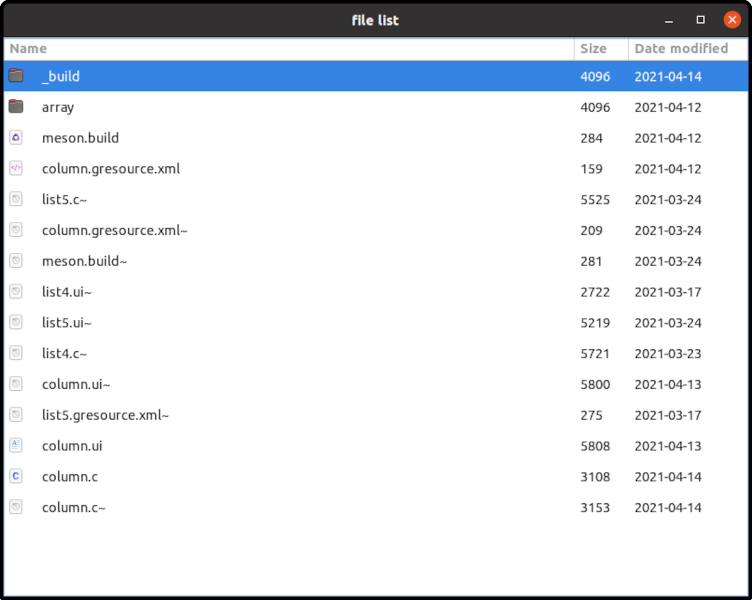
\includegraphics[width=11.3cm,height=9cm]{../image/column_view.png}
\caption{Column View}
\end{figure}

If you click the header of a column, then the whole lists are sorted by
the column. If you click the header of another column, then the whole
lists are sorted by the newly selected column.

GtkColumnView is very useful and it can manage very big GListModel. It
is possible to use it for file list, application list, database frontend
and so on.
